
% Outline

% introduce EDRs and how they are used to protect organisations

% introduce process injection attacks: MITRE, and NT process attacks

% how do EDRs

%\section{Proess Injection Attack and EDR Repsonse Primer}
\pagebreak
\section{The evolving threat landscape of process injection}

Malware attacks using code injection predates modern Windows operating systems, with the first notorious example probably being the ``Moris Worm''
that targeted UNIX systems in 1988, by exploiting a buffer overflow bug \autocite{Spafford:1989}.  This remote exploit has several
traits that malware writers still try to find; it executes at the privilege level of the service being attacked and there is no complicated
thread execution needed to initiate.

The history of the code injection techniques used by Windows malware could be argued to have started with more altruisic motives.
Microsoft themselves patented a method to map an external module into a target process in 2004 \autocite{Ghizzoni:2004}.  This has the
stated aim of, somewhat ironically supporting applications such as ``anti-virus programs, profilers, debuggers, and pseudo-localization testing''.

And the race was then on to determine whether a program utilising these dynamic-link library (DLL) loading methods were malicious.
The first malicious code detection methods would judge the motives by looking at static evidence within the program file itself,
with checks based on code signing, file metadata, Portable Executable (PE) file header analysis, etc. \autocite{Jang:2007}.

\subsection{Code Injection Taxonomy}

To understanding the general principles, it is helpful to use the taxonomy of \textcite{Barabosch:2014}.
The authors distinguish between Host-Based Code Injection Attacks (HBCIA) that orginate and infect process on the
same system from Remote-Based Code Injection Attacks (RBCIA), such as worms, where the victim process is on a system
remote from the infecting agent.

They then neatly summarise the HBCIA into three steps that we will see when we meet Mockingjay:

\begin{enumerate}
\item selecting a victim process,
\item copying code into the victim process, and
\item executing the injected code.
\end{enumerate}

\begin{figure}[ht]
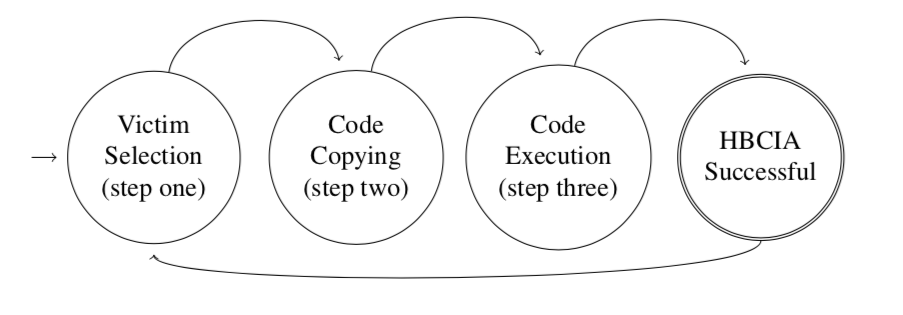
\includegraphics[scale=0.4]{hbcia_3step_algo.png}
\caption{HBCIA Attack Steps \autocite{Barabosch:2014}}
\end{figure}


How we select our victim and how we execute our code can be categorised to aid our understanding of attack methods as:

\begin{itemize}
\item Victim Selection:
  \begin{enumerate}
  \item Targeted Injection:
    \begin{itemize}
    \item Malware selects a specific subset of processes to inject into based on an internal target list (e.g., critical
        processes like explorer.exe.)
    \item Less suspicious as avoids risky/unnecessary processes.
    \end{itemize}
  \item Shotgun Injection:
    \begin{itemize}
    \item Greedy approach that blindly injects itself into as many accessible processes as possible.
    \item More suspicious as may accidentally target antivirus or risky processes.
    \end{itemize}
  \end{enumerate}
\item Code Execution:
  \begin{enumerate}
  \item Concurrent Execution:
    \begin{itemize}
    \item The injected code runs in parallel with the original code in the victim process, with original process continue executing.
    \item Additional threads are spawned for the injected code.
    \end{itemize}
  \item Thread Manipulation:
    \begin{itemize}
    \item The injected code replaces or blocks the original victim process's thread(s) which do not continue.
    \item Victim process exhibits mainly the injected code's behaviour.
    \end{itemize}
  \end{enumerate}
\end{itemize}

\begin{table}[!ht]
  \centering
  \caption{Prevalence of classes of HBCIA algorithms \autocite{Barabosch:2014}}
\begin{tabular}{ |p{2cm}|p{2.5cm}||p{4.2cm}|p{4.2cm}|  }
  \hline
  & & \multicolumn{2}{|c|}{Victim Selection} \\
  \cline{3-4}
  & & Targeted Injection & Shotgun Injection \\ 
  \hline
  \hline
  Code  & 	Concurrent  & TICE 58\% & SICE 23\% \\
  Execution & Execution &  Hanthie (Linux) & Flashback (Mac OS X) \\
  \cline{2-4}
  &  Thread  & TITM 20\%  & SITM: 00\% \\
  & Manipulation & Stuxnet (Windows) &  \\
  \hline
\end{tabular}
\label{table: HBCIA}
\end{table}


\subsection{Common techniques in windows malware attacks}

When understanding the possible approaches to protecting against code injection attacks researchers look at all classes of attacks.
MITRE ATT\&CK\textregistered\; is a knowledge base of advesary tactics which is a useful resource and collects information on injection implementations
for all major OSs, with a dizzing array of samples \autocite{Mitre:2017}.

A more useful summary when understanding the Mockingjay attack is to look at the common Windows techniques \autocite{Hosseini:2017}.  We
can follow a line of evolution in newer attacks, from the classic DLL injection method, to file-less methods, and newer methods that
avoid telltail behaviours of older techniques.

\begin{table}[!ht]
\centering
\caption{10 Windows Process Injection Techniques. Reproduced from \autocite{Hosseini:2017}}
\begin{tabular}{ |p{3.5cm}||p{10.5cm}|  }
  \hline
  \multicolumn{2}{|c|}{Ten process injection techniques} \\
  \hline
  Name & Description \\
  \hline
  Classic DLL Injection Via Createremotethread and Load Library
             & The malware writes the path to its malicious DLL in the virtual address space of another process,
               and ensures the remote process loads it by creating a remote thread in the target process. \\
  \hline
  PE Injection
             & Copy malicious code into an existing open process and cause it to execute (either via a
               small shellcode, or by calling CreateRemoteThread). The malware is file-less, not placing a malicious DLL
               on the disk.  It still allocates memory in a host process (e.g., VirtualAllocEx),
               but writes its malicious code by calling WriteProcessMemory. \\
  \hline
  Process Hollowing (A.K.A Process Replacement and Runpe)
             & The malware unmaps (hollows out) the legitimate code from memory of the target process and
               overwrites the memory space of the target process (e.g., svchost.exe) with a malicious executable.\\
  \hline
  Thread Execution Hijacking A.K.A Suspend Inject and Resume (SIR)
             & After getting a handle to the target thread, the malware puts the thread into suspended mode by
               calling SuspendThread to perform its injection. The malware calls VirtualAllocEx and
               WriteProcessMemory to allocate memory and perform the code injection. Targeting an existing thread
               of a process, during analysis you will probably see calls to CreateToolhelp32Snapshot and
               Thread32First followed by OpenThread. \\
  \hline
  Hook Injection via Setwindowshookex
             & Malicious DLL loaded upon an event getting triggered in a specific thread. This is usually
               done by calling SetWindowsHookEx to install a hook. \\
  \hline
  Injection and Persistence via Registry Modification (e.g. Appinit\_DLLS, AppCertDLLs, IFEO)
             & Appinit\_DLL, AppCertDlls, and IFEO (Image File Execution Options) are all registry keys that
               malware uses for both injection and persistence. \\
  \hline
  APC Injection and Atombombing
             & Use APC to force another thread to execute their custom code by attaching it to the APC
               Queue of the target thread. \\
  \hline
  Extra Window Memory Injection (EWMI) via Setwindowlong
             & Injecting into Explorer tray window’s extra window memory and has been used a few times
               among malware families such as Gapz and PowerLoader. There is not much room in EWM, so the
               malware writes code into a shared section of explorer.exe and uses SetWindowLong and
               SendNotifyMessage to have a function pointer to point to the shellcode, and then execute it. \\
  \hline
  Injection Using Shims
             & Shims allow developers to apply fixes to their programs without the need of rewriting code.
               Malware can take advantage of shims to target an executable for both persistence and injection.
               Windows runs the Shim Engine when it loads a binary to check for shimming databases
               to apply the appropriate fixes. \\
  \hline
  At Hooking and Inline Hooking (A.K.A Userland Rootkits)
            & Malware changes the import address table. When a legitimate application calls an API located
              in a DLL, the replaced function is executed instead of the original one. \\
  \iffalse
\fi
  \hline
\end{tabular}
\label{table: ProcessInjectionTechniques}
\end{table}


\subsection{End-point security}

EDR solutions cover a wide range of cyber-security capabilities to monitor in real time the health of applications
and services, detect anomalous activity and respond to an attack.
Related technologies are Managed Detection and Response (MDR) \autocite{Hayes:2023}, which offers end-point security as a service, and
eXtended Detection and Response, which consolidates applications and collects data from across the enterprise to
have a wider scope of view to detect changes in behaviours across systems.

For the rest of this report, we will not delve into the specifics of the capabilities of the various end-point solutions.
But we can use the MITRE categories to see where these defences are focused:


\begin{table}[!ht]
  \centering
  \caption{Attack Mitigants \autocite{Mitre:2017}}
\begin{tabular}{ |p{1.2cm}||p{2cm}|p{10.2cm}|  }
  \hline
  \multicolumn{3}{|c|}{PI Mitigation List} \\
  \hline
  ID	& Mitigation & Description \\
  \hline
  M1040	& Behaviour Prevention on End-point &	End-point security solutions can be configured to block some types of
                                            process injection attacks by monitoring certain API calls
                                            and observing tell tail sequences of behaviour that occur during the
                                            injection process.  Attack Surface Reduction (ASR)
                                            rules may prevent code injection into Office applications.\\
  \hline
  M1026 & Privileged Account Management	& Restrict the use of certain applications that can be abused by
                                          process injection to privileged users only. Apply and monitor: advanced access control and
                                          process restrictions. \\
  \hline
\end{tabular}
\label{table: Mitigations}
\end{table}


\subsection{Deploying a file-less payload into Windows memory space}

The Nirvana callback is a method Microsoft developed to control a running process with needing to recomplie or rebuild code.
It inserts a user mode function to be called on the return from a kernel system call.
Originally developed as a legitimate instrumentation technique,
it is important to our discussion as it has been used to allow malware payloads to be delivered directly into the
address space of a running process \autocite{Dequeker:2023}.

An attacker loads a payload into the RWX section then registers a Nirvana callback to execute the call after the normal program
execution makes a system call.

\begin{figure}[ht]
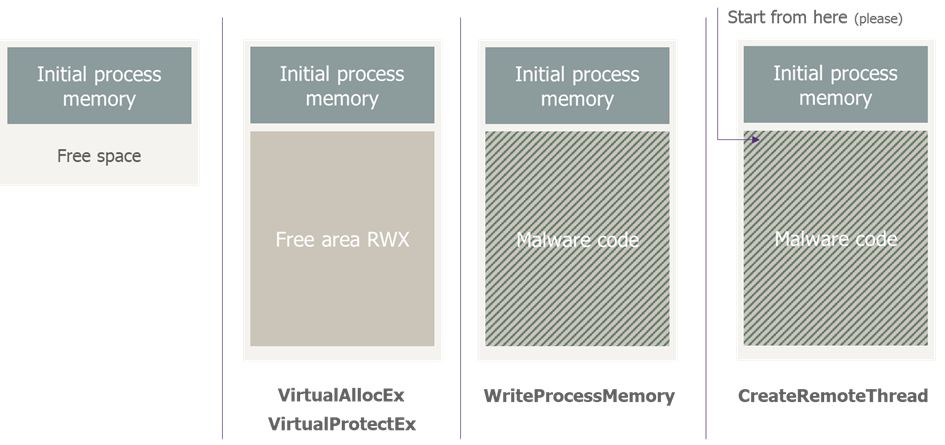
\includegraphics[scale=0.9]{dequeker_standard_process_injection_pattern.png}
\caption{RWX process Injection pattern \autocite{Dequeker:2023}}
\end{figure}
 
The direct attack can be detected by an EDR/XDR as it needs to use the monitored NtSetInformationProcess call.  But the pattern
will be adapted by Mockingjay.

%\subsection{Use cases for process injection in malware}

%\subsubsection{Evading detection}

%\subsubsection{Privilege escalation}

%\subsubsection{Payload delivery and execution}

%\subsubsection{Deploying Payload into Windows Memory Space}

% \href{https://modexp.wordpress.com/2018/07/15/process-injection-sharing-payload/}{Process injection sharing payload}


%\autocite{Zhan:2018}

%\href{https://www.riskinsight-wavestone.com/en/2023/10/process-injection-using-ntsetinformationprocess/}{PI using NTSetInformationProcess}

%\href{https://github.com/elddy/Windows-NTAPI-Injector}{NTAPI injector} 

%\href{https://gist.github.com/WKL-Sec/96e17188e4c159c2cdf7ff2c111130cc#file-local-c}{Injector examples in C}

%\href{https://www.unknowncheats.me/forum/anti-cheat-bypass/286274-internal-detection-vectors-bypass.html}{internal detection vectors bypass}

%\href{https://medium.com/@s12deff/process-injection-with-random-rwx-memory-spaces-3e3651149527}{PI with random RWX memory spaces}


%\subsection{Detection and Mitigation}

%\subsubsection{Current strategies for detecting process injection}

%\subsubsection{Anti-malware tools and techniques}

%\subsubsection{Best practices for preventing and mitigating process injection attacks}

%\begin{itemize}
%\item DLL Injection
%\item Code Injection
%\item Atom Bombing
%\item Reflective DLL Injection
%\end{itemize}


\subsection{EDRs response to an evolving threat landscape}

EDR/XDR cyber-security solutions have been incorporating protections of increasing levels of sophistication.

At the first level, as discussed earlier, there are static monitoring of a specific machine DLLs and processes to detect changes.  They also
make sure that certain subsystems have not been modified, have elevated permissions, or that there are unknown processes
running on the monitored system.

Next, user and entity behaviour analytics (EUBA) tools identify changes in behaviours that could indicate a threat.  This could include the
applications and systems a user normally uses, looking for configuration changes, and scanning log files for changes in behaviour.  Statistical
modelling will profile normal activity and continuous monitoring will attempt to discern anomalous behaviour if a threat occurs.

Researchers are now looking to detect process injection using fine-grained analysis of API call chains using deep learning \autocite{Wang:2022}.

Anomaly detection can be prone to false positives.  The threat actor will look for attacks that could look like innocent behaviour.

The response is to use increasingly sophisticated AI and machine learning techniques by looking at system entity interactions.  The behaviours
of interest to detect potential threats are complicated to the extent that rules based systems relying on expert knowledge to set up tend to
be brittle.

Looking at behaviours as connected system operations, some methods involve the inference of intent from audit logs
and the clustering of semantically similar behaviours \autocite{Zeng:2021}.
Causal analysis technologies are looking at data provenance as a way to improve detection rates \autocite{Inam:2023}.
An example of this is in a paper by \textcite{Zengy:2022} where providence analysis of system auditing records is used to
search for anomalies that an attack would produce.  


Even as end-point detection solutions broaden and deepen their approaches, we can still envisage a series of adaption and evasion moves that
leaves total cyber-protection an ideal that cannot always be realised. 


%End-point Detection and Response Systems (EDR) have developed to counter these myriad threats.  These systems are gaining in sophistication and adversaries
%are on the hunt for new ways to evade these systems.

%In this report we look at a new variation of one attack technique, process injection, and ask how EDRs protect against these attacks and how
%this new technique would evade those barriers.  In particular we are looking at the ``Mockingjay'' attach that targets modern Windows machines.

%These protections can be signatu


% \href{https://www.crowdstrike.com/cybersecurity-101/endpoint-security/edr-vs-mdr-vs-xdr/}{EDR vs MDR vs XDR}
%HBCI techniques work on injecting code into running processes and having that code executed as part of the normal process
%execution.  End-point Detection and Response (EDR) systems \autocite{Hayes:2023} provides realtime visibiluty

%Process injection seeks bypass EDR hooks by injecting code into trusted processes with RWX permissions already set.

%\subsection{Emerging trends in malware attacks on Windows}

%\subsection{Advancements in process injection techniques}

%\subsection{Future predictions for the evolution of these threats}


